%\documentclass{sig-alternate}
\documentclass{ueacmpstyle}

\newenvironment{quoted}{\begin{quotation}\it}{\end{quotation}}
\usepackage{hyperref}
% Prevents author/year errors
\usepackage{natbib}
\usepackage{float}
\usepackage{rotating}
\usepackage[strings]{underscore}
\renewcommand{\paragraph}[1]{\par\textbf{#1}\hspace{0.3em}}
\setlength{\parskip}{0.5em}


\begin{document}


\title{Transport+ \\ Developing an Accessible and Usable Website Application }

\author{
James Campbell and Debbie Taylor \\ 100017655 and 100085169
}

\maketitle

\begin{abstract}
	Technology is expanding at an ever increasing rate and is now used by everyone from young children to senior citizens and disabled people. This means website applications (apps) must be developed to cater for the needs of everyone. Transport+ is a website app designed specifically to showcase usability and accessibility.
\end{abstract}

\section{Introduction} 
Website apps must be accessible to experienced users but also easy to use and have built in help features for those that are new and/or inexperienced. Accessibility can cover disabilities but can also affect all users, not just disabled ones. `These design concerns must be considered if both the users' experience and business objectives are to be met' \citep{petrie2004tension}.
 
Usability is a way of identifying and assessing how easy website interfaces are to use. The word `usability' refers to methods for improving ease-of-use during the design process and key design functionality is: Does it do what users need and is it easy to interact with? \citep{lee2012understanding}.

To develop Transport+, the first stage was to produce a basic site, then build in both accessibility and usability. This has been challenging as these two functionalities can sometimes contradict each other, for example a larger font size makes the site accessible to visually impaired users but, if it's too big, it can cause usability issues for normal sighted users. 

This report will discuss how the authors' built Transport+ to be accessible and usable for everyone.

\section{Investigating Accessibility and Usability}
Firstly the authors' investigated if there were any rules and/or guidelines around accessibility and usability:

\subsection{Accessibility}
In May 1999 the Web Content Accessibility Guidelines (WCAG) were published to provide `general and specific guidance'
to Web developers for assessing and ensuring the accessibility of their content \citep{world2008web}. These have been updated several times since then and the authors' used these guidelines to ensure their site was accessible to a wide range of people with disabilities.

\subsection{Usability}
In 2003 the `U.S. Department of Health and Human Services’ (HHS) Research-Based Web Design and Usability Guidelines' were published to identify innovative, research-based approaches resulting in easy-to-use websites \citep{leavitt2006based}. 

These helped the authors' identify issues any designer needs to consider when planning and designing a website, such as: clear and concise goals, clear user requirements, ensuring websites meet user’s expectations, setting usability goals, and providing useful content.

It is clear both these functionalities are fundamental to designing a working website application. If either of these are ignored it considerably reduces who can use the site and whether or not a user will revisit the site after their first experience.

Once both these guidelines were identified and investigated it was time to start developing the Transport+ website app, using the below scenario design and scenario.

\section{Scenario Design}
The intended users for the Assignment 2 website are customers wishing to view travel arrangements for a trip, using different modes of transport across their whole journey eg. bus and train from Wymondham to London. Their computer literacy range will cover basic through to expert level, with some disabilities and they will use the website to:

\begin{itemize}
	\item View timetables
	\item Plan a journey using different modes of transport
\end{itemize}

\subsection{Scenario}
To develop the scope and functionality needed for Transport+, we used the following scenario, to `walk in a users shoes' and fully understand what is required:

\begin{quoted}
\noindent{I'm a 70 year old lady. I'm dyslexic, got glaucoma and I'm retired. }

I like to travel but this trip will be to visit my son who lives in London. I'm not very good with technical gadgets, so need something easy to use and understand, especially due to my dyslexia and visual impairment.
 
I want to be able to find my travel details really easily and I don't want lots of distracting adverts or lots of different places I have to work through to find what I need. The information needs to be clear and precise. My dyslexia means I struggle to understand long and complex instructions and comments, so short simple comments and instructions are much better for me. 
My glaucoma means I need an easy to view website with writing that is big enough for me to understand.

I will be accessing this site at my local library so it needs to be quick and have no delays, as I will be restricted to getting this done within the timeslot I am allocated. 
I will also need to access this when I visit my son in London, so I will need it available late at night (he works very hard and often is not home until about 10pm).	

I want to be able to see live updates of what trains and buses are available, at any time of the day.
\end{quoted}


\section{Design}
Transport+ has been designed to provide transport information for any area of the United Kingdom, while being accessible and usable to anyone, including people with disabilities. The design is very clean and crisp without any extraneous features that could distract from the information it provides. 

It enables a user to select train, bus and taxi information and see a list of which options are available at the time it is requested, eg it refreshes as and when the transport information is updated by the relevant transport companies (see appendix 1 for the homepage).

The site makes use of the Usability HHS and Accessibility WCAG guidelines to ensure it's fit for purpose and caters to the needs of everyone. It is also built to take into account Jakob Nielsen's ten Usability Heuristics \citep{DBLP:books/lib/Nielsen00};

\begin{itemize}
	\item Visibility of system status
	\item Match between system and the real world	
	\item User Control and freedom
	\item Consistency and standards
	\item Error prevention
	\item Recognition rather than recall
	\item Flexibility and efficiency of use
	\item Aesthetic and minimalist design
	\item Help users recognise, diagnose and recover from errors
	\item Help and Documentation
\end{itemize} 

For example the site is built with consistency across all pages, with an input box in the middle for recognition and recall and there are help functionalities that can be understood by both standard users and the visually impaired. A full breakdown of the design, usability and accessibility functionalities are below. 

\subsection{Developers and Designers}
Human Computer Interaction is very important for user accessibility and usability, however, it is equally important for Developers and Designers. They need to fully understand the impacts of both in order to design, develop and deliver the optimum user experience for all user abilities. Without this knowledge they would produce a website app that would be effective for some of the population but would discriminate against the most vulnerable in society.

If a website is designed and developed to work for people with disabilities then it will also work for the majority of standard users, however, there is a balance needed. If usability and accessibility are treated as a check-box process then the human interaction aspect can be lost.

\subsection{Prototypes and Diagrams}
Before starting the actual development stage the authors produced a low fi prototype and UML diagram to help them understand the proposed website app (see appendix 2 and 3). These were needed to identify the scope of the project, the functionalities required and how it all fit together.

\section{Description, Usability and Accessibility Functionalities}
\noindent{\textit{\textbf{{Usability}}} features incorporated into the design enable a user to input a station in the train section, a code in the bus section and the taxi section shows the top taxi firms available and their contact details, along with a map to show where they are based. 

The information is input via a text box in the middle of the page and this is the only information that is needed, due to the website using the current date and time to show the next available option eg if the user wishes to select train options from Wymondham they just input the three letter station code WYM, but if they want to access London Liverpool Street Station they use LST (see appendix 4).    
 
For the buses they need to input the Association of Transport Coordinating Officers (ATCO) code eg for a single Wymondham bus stop this is 2900W5854 and the site has a built in link to find whichever bus stop ATCO code is required (see appendix 5). 
 
If the user is unsure what to do they can click the built in help feature and this will inform them what to do (see appendix 6) This has been produced using visual and text instructions, so it's easy to understand, no matter what level of disability or technical knowledge the user has.

The site has been designed so nothing requires a double click, therefore making it easy to use for people with mobility issues. For example if you click on the `Go` button it won't keep duplicating the list, it will only change if the time and/or options have changed.

\noindent{\textit{\textbf{{Accessibility}}} features start by the authors increasing the Text Font size from the standard 12px-18px to a larger 30px, to ensure it can be read by everyone, without it being too big for standard users.

The next relates to the main colour scheme being monochrome. This eliminates any issues with colour blindness or visual impairment but is still pleasing to the eye for standard users.

There is also the option to select an `Accessibility' button to change the background colour to dark blue, with white text, rather than the monochrome, in case the user is acutely visually impaired and/or dyslexic. (see appendix 1) 

There is an overlay `help' feature to show which fields to complete and how to use them (see appendix 6).

The authors' tested the website layout and colour contrasts via the WCAG 2.0 checker and the layout achieved AA and the colour contrast received AAA (AAA being the top score available). Transport+'s contrast ratio of 11.31 is also much higher than the standard required AAA ratio of 7 (see figure 1 below)

\begin{figure}[H]
	\centering
	\begin{tabular}{ll}
				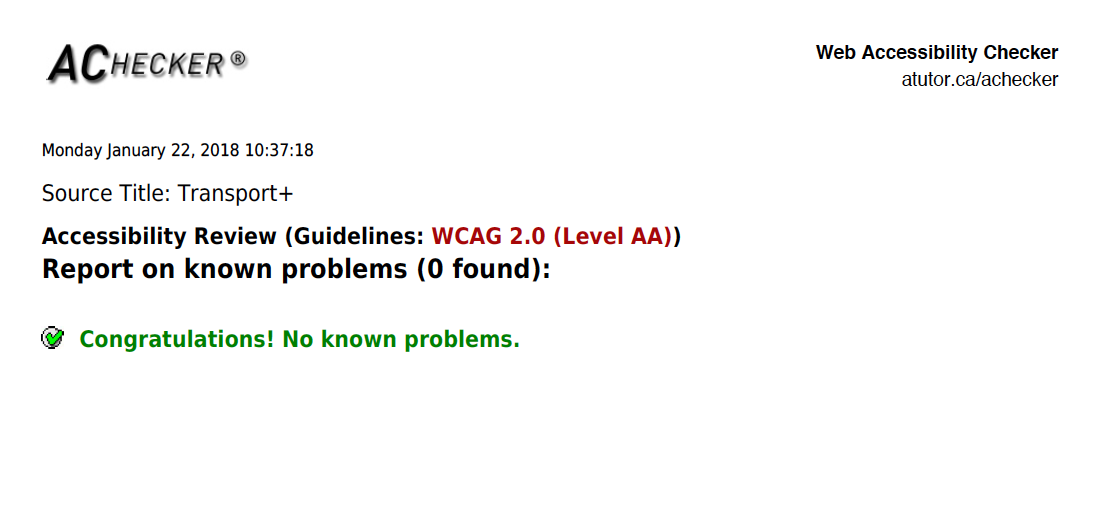
\includegraphics[trim=0cm 0cm 0cm 0cm, clip=true, totalheight=0.2\textheight, angle=0]{photos/access_rating.png}
		&
				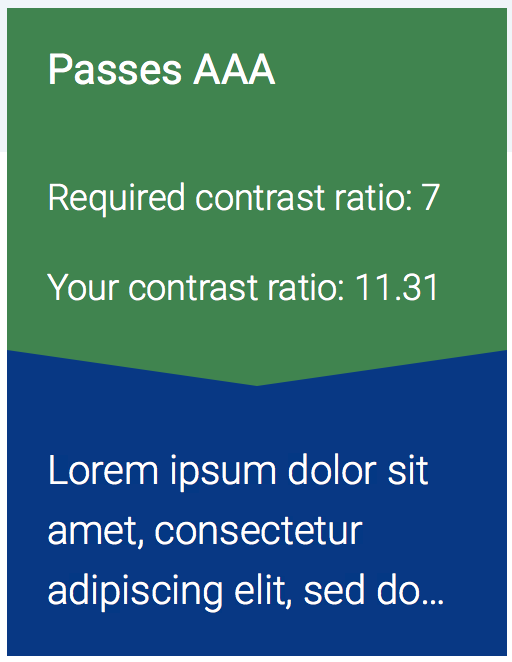
\includegraphics[trim=0cm 0cm 0cm 0cm, clip=true, totalheight=0.2\textheight, angle=0]{photos/colour_rating.png}
	\end{tabular}
	\caption{WCAG 2.0 Website App ratings}
\end{figure}
	
\subsection{Trade-Offs}
The main trade-off for the website is that there's no ability to select `To and From' in any section. This would have created a website that was more complex and difficult to use for people with disabilities or technologically inexperienced. 

The remit was to create a website app that gives travel information, therefore, the authors decided it was better to produce a functional easy to use site, rather than an overcomplicated version. 

This means that if someone is very experienced and has no disabilities they may find the site a bit too easy to use, but it will still provide them with the information they require.

If this project were to move into a future iteration it could easily be adapted to include more detailed and complex search functions.

\section{Evaluation}

The site has been evaluated using the same Don Norman design principles as coursework 1 \citep{rogers2011interaction}. They are:

\paragraph {Visibility}\textit{The more visible functions and operations are, the more likely users will be able to know what to do.}
\paragraph{Feedback}\textit{Information passed back to user about what action has been done and what has been accomplished. This allows the user to continue with the activity.} 
\paragraph{Constraints}\textit{Enabling restrictions for user interaction at a given moment.} 
\paragraph{Mapping}\textit{Relationship between controls and their effects eg. up and down arrows used to represent the up and down movement of the cursor on a keyboard.}
\paragraph{Consistency}\textit{Interfaces having similar operations and elements for achieving similar tasks eg always clicking the Enter button to select.} 
\paragraph{Affordance}\textit{An attribute of an object that allows people to know how to use it. eg. mouse button being pushed.}

The authors tested the website app themselves and gave a rating out of ten for each principle. They then asked Mary, who has zero technical knowledge, to test the site and rate each of the principles, followed by Vicky who is visually impaired. See table 1 below for each set of ratings:

\begin{table}[h!]
	\centering 
	\caption{Evaluation results using Norman's Principles}\label{textresult}
	\begin{tabular}{|lrrrrrrr|} \hline
		\textit{Testers} & \textit{Visibility} & \textit{Feedback} & \textit{Affordance} & \textit{Mapping} & \textit{Constraints} & \textit{Consistency} & \textit{Total} \\
		Authors & 8.5/10 & 7/10 & 7.5/10 & 9/10 & 9/10 & 9/10 & 50/60 \\
		Mary & 8/10 & 8/10 & 7/10 & 8/10 & 9/10 & 8/10 & 48/60 \\
		Vicky & 8/10 & 8/10 & 8/10 & 9/10 & 9.5/10 & 9.5/10 & 52/60 \\
		\hline
	\end{tabular}
\end{table}

The authors rate this as 83 percent, Mary gives it 80 percent and Vicky's score is 86.6 percent. This shows the authors have produced a website that is usable for all and supports the outcome of the WCAG 2.0 checker. 

The major issues identified while building the website app have been juggling disability needs verses standard users. Some disabilities require certain colours whereas others need different ones. It took a lot of investigation to identify the base monochrome and blue disability accessibility colours as ones that could be used by everyone.

As the site was designed to be very easy to use it is possible some experienced users, without disabilities, may see it as too basic for their needs, even though it does provide everything in the remit. This could be improved during future iterations of the website app, but this currently covers the majority of common disabilities and basic to mid-range users.  

\section{Conclusions}
The authors have concentrated on ensuring Transport+ is a website app that is usable and accessible to everyone, but caters more for disabilities than experienced users. 

The  Usability HHS and Accessibility WCAG guidelines were closely followed and this produced a site that is rated highly by both visually impaired and technologically inexperienced users.

When comparing the results, and asking for feedback from the testers, they confirmed the website application is fit for purpose. They are happy with the straightforward, clean and easy to use site and stated they preferred this to a much more complicated one. Vicky, especially, likes the separate accessibility option, as this makes it much easier for her to read and use.

In the future, the authors would continue with the same theme, but would add in more functionality while ensuring the site stays easy to use and accessible to everyone.







\bibliographystyle{apalike}
\bibliography{hci}  

\end{document}
